\documentclass{article}

\usepackage{hyperref} % Almost certainly will need
\usepackage{fullpage} % Good for making PDFs as well
\usepackage{listings} % Needed to insert code
\usepackage{lstautogobble}
\usepackage{float}
\usepackage{graphicx}

\usepackage[T1]{fontenc}
% This makes it so the web pages don't have indents as most of the time
% they are just annoying
\setlength{\parindent}{0pt}

\usepackage{textcomp}
\lstset{
  upquote=true,
  basicstyle = \ttfamily,
  columns=fullflexible
  escapeinside=||,
  autogobble
}



% This section allows for tex4ht only control statements
% From http://tex.stackexchange.com/questions/93852/what-is-the-correct-way-to-check-for-latex-pdflatex-and-html-in-the-same-latex
\makeatletter
\edef\texforht{TT\noexpand\fi
  \@ifpackageloaded{tex4ht}
    {\noexpand\iftrue}
    {\noexpand\iffalse}}
\makeatother

\newcommand{\code}[1]{\texttt{\textmd{#1}}}
\newcommand{\assertion}[2]{\textbf{Assertion: }#1 (\hyperlink{#2}{#2})}
\newcommand{\assertionref}[1]{\hyperlink{#1}{#1}}
\newcommand{\assertiondest}[1]{\hypertarget{#1}{\textbf{#1}:}}
\newcommand{\clarification}[2]{\textbf{Clarification: }#1 (\hyperlink{#2}{#2})}
\newcommand{\clarificationdest}[1]{\hypertarget{#1}{\textbf{#1}:}}

\usepackage[usenames]{color}
\newif\ifComments
\Commentstrue

\ifComments
\newcommand{\todo}[1]{\noindent\textcolor{red}{{#1}}}
\newcommand{\chek}[1]{\noindent\textcolor{red}{Check: {#1}}}
\newcommand{\nelson}[1]{\noindent\textcolor{blue}{Nelson: {#1}}}
\newcommand{\marcus}[1]{\noindent\textcolor{BurntOrange}{Marcus: {#1}}}
\else
\newcommand{\todo}[1]{}
\newcommand{\chek}[1]{}
\newcommand{\nelson}[1]{}
\newcommand{\marcus}[1]{}
\fi

\begin{document}

% This is an SCalc of using a switch to have pdf/html only code
\ifpdf
  \LARGE
  \textbf{SCalc}
  \normalsize
\fi

The goal of this assignment is to implement a compiler for a simple imperative language called
\textit{SCalc}. This compiler will directly generate code for the following three backends:
\begin {itemize}
  \item \textit{x86} assembly
  \item \textit{MIPS} assembly
  \item \textit{ARM} assembly
\end {itemize}
You must also create an \textit{interpreter} for \textit{SCalc}

For the interpreter you will be computing the value of the expressions as you traverse the tree.
However, when generating assembly code for each of the backends \textbf{you are not allowed to
perform any computations in the compiler}. You must create assembly code to perform all of the
computations that appear in the input file.

\textit{MIPS} assembly will be run using \textit{SPIM}\\
\textit{x86} assembly will be assembled using the nasm assembler and run natively.\\
\textit{ARM} assembly will be compiled using the \textit{ARM} toolchain (assembler
\code{arm-none-eabi-as}, linker \code{arm-none-eabi-gcc}) and then run using an \textit{ARM}
simulator (\textit{qemu-arm}).

Your compiler will produce the assembly text files, not binaries. \textbf{You must generate your
assembly using \href{https://github.com/pantor/inja}{\textit{inja}}}. Inja is a string template
engine which allows you to make use of formatted strings. Its syntax is similar to
\textit{Python}'s jinja. You won't need any advanced features to complete this assignment.

Your classes should follow a pattern of classes matching the following UML diagram (structure only,
names should be reasonably changed):
\begin{figure}[H]
  \centering
  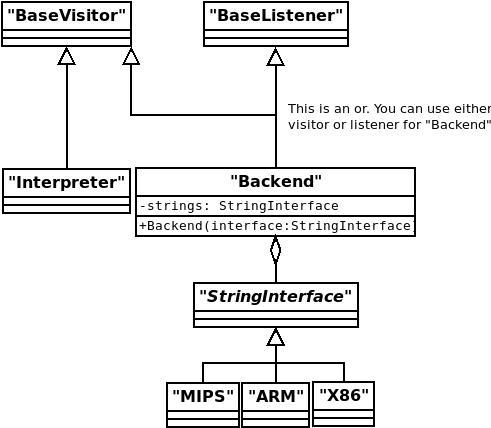
\includegraphics{static/expectedForm.png}
\end{figure}

Note that you must use the visitor pattern for the interpreter as it is impossible to revisit nodes
during a loop when using the listener pattern.

Beyond these constraints you are allowed to use any internal representation that you wish, as well
as emit any code that you wish, as long as the output is correct.

\section{Language Specification}
\textit{SCalc} has integer variables, conditionals, loops, prints, and various integer expressions.

\subsection{Reserved Keywords}
The following Keywords are reserved in \textit{SCalc}:
\begin {itemize}
  \item{\code{if}}
  \item{\code{fi}}
  \item{\code{loop}}
  \item{\code{pool}}
  \item{\code{int}}
  \item{\code{print}}
\end {itemize}

\subsection{Booleans}
In this assignment, booleans can only be produced using comparison operators, there is no literal to
express them. As well, they are ephemeral: there is no way to store them. They can only exist when
created using one of the comparison operators.

When printed, booleans take on a value of 1 (true) or 0 (false). For example:
\begin{lstlisting}
  print(1 == 1);
  print(1 == 0);
\end{lstlisting}
produces the following output:
\begin{lstlisting}
  1
  0
\end{lstlisting}

As well booleans \textit{are} usable in expressions and must be \textit{upcast} to an integer.
This means if a boolean is used in an arithmetic expression it takes on the integer value described
above. For example:
\begin{lstlisting}
  print(1 + (1 == 1));
  print(1 + (1 == 0));
\end{lstlisting}
produces the following output:
\begin{lstlisting}
  2
  1
\end{lstlisting}

\subsection{Integers}
In this assignment, integers are the \textit{only} numerical type (there is no floating point type).
As well, they are the only type that you can store.

In this assignment integer literals are defined as being a string that contains only the numerals
0-9 with no spaces.

\assertion{All integer literals will be $\geq 0$.}{nonnegative-literals}\\

Examples of valid integers:
\begin{lstlisting}
  1
  123
  5234
  01
  10
\end{lstlisting}

Examples of invalid integers:
\begin{lstlisting}
  1.0
  one
  1_1
  1o
\end{lstlisting}

As well, integers \textit{are} usable in conditions and must be \textit{downcast} to booleans. This
means in a condtional, an integer that \textit{is not} zero will be considered true and an integer
that \textit{is} zero will be considered false. For example:
\begin{lstlisting}
  if (999)
    print(999);
  fi;
  if (0)
    print(0);
  fi;
\end{lstlisting}
produces the following output:
\begin{lstlisting}
  999
\end{lstlisting}

\subsection{Identifiers}
For the purpose of this assignment, identifiers are simple. They must start with an alphabetical
character. This character may be followed by numbers or alphabetical characters. A keyword cannot
be used as an identifier.

Examples of valid identifiers:
\begin{lstlisting}
  hello
  h
  h3llo
  Hi
  h3
\end{lstlisting}

Examples of invalid identifier:
\begin{lstlisting}
  3d
  a-bad-variable-name
  no@twitter
  we.don't.like.punctuation
  or_spelling
\end{lstlisting}

\subsection{Expressions}
An expression is composed of integers, identifiers, and operators.

\subsubsection{Operators}

\begin{center}
  \begin{tabular}{|c|l|c|l|c|}
    \hline
    \textbf{Class} & \textbf{Operation} & \textbf{Symbol} & \textbf{Usage} &
    \textbf{Associativity} \\
    \hline
    Arithmetic
    &addition      & + & \texttt{expr + expr} & left \\
    &subtraction    & - & \texttt{expr - expr} & left \\
    &multiplication & * & \texttt{expr * expr} & left \\
    &division       & / & \texttt{expr / expr} & left \\
    \hline
    Comparison
    &less than      & <  & \texttt{expr < expr}  & left \\
    &greater than   & >  & \texttt{expr > expr}  & left \\
    &is equal       & == & \texttt{expr == expr} & left \\
    &is not equal   & != & \texttt{expr != expr} & left \\
    \hline
  \end{tabular}
\end{center}

\clarification{There is no remainder operator in SCalc.}{no-rem}\\
\clarification{There is no exponentiation operator in SCalc.}{no-pow}\\
\clarification{Division is integer division.}{int-div}\\

\subsubsection{Valid Expressions}
Valid formats for expressions are
\begin{lstlisting}
  (<expr>)
  <expr> <op> <expr>
  <int>
  <id>
\end{lstlisting}

\begin{itemize}
  \item \code{expr} is an expression.
  \item \code{int} is an integer.
  \item \code{id} is the identifier of a variable.
\end{itemize}

\assertion{All expressions will result in a value that fits in a 32 bit signed integer.}
{expression-size}\\
\assertion{No expression will contain a division by 0.} {zero-divide}

Examples of valid expressions are
\begin{lstlisting}
  i * 2 * 10 + 4
  2 - 4 * 5
\end{lstlisting}

\subsubsection{Precedence}
Precedence determines what order operations are evaluated in. Precedence works as defined in the
following table:
\begin{center}
  \begin{tabular}{|c|c|}
  \hline
  \textbf{Precedence} & \textbf{Operations} \\
  \hline
  HIGHER
  & *,/ \\
  & +,- \\
  & <, > \\
  LOWER & ==, != \\
  \hline
  \end{tabular}
\end{center}

\subsection{Statements}

In \textit{SCalc} there are five types of statements:

\begin{itemize}
  \item \hyperref[sssec:declaration]{declaration}
  \item \hyperref[sssec:assignment]{assignment}
  \item \hyperref[sssec:conditional]{conditional}
  \item \hyperref[sssec:loop]{loop}
  \item \hyperref[sssec:print]{print}
\end{itemize}

Each statement ends with a semicolon. White space is not important in \textit{SCalc}.

\assertion{Whitespace is guaranteed to be a space, a tab, a carriage return, or a new
line.}{simple-whitespace}

\subsubsection{Declaration}
\label{sssec:declaration}
A variable declaration in \textit{SCalc} has the following form:
\begin{lstlisting}
  int <id> = <expr>;
\end{lstlisting}

\begin{itemize}
  \item \code{id} is the identifier of a variable.
  \item \code{expr} is an expression.
\end{itemize}

Variables have a few properties:\hypertarget{variable-props}{}
\begin{itemize}
  \item cannot be used before being declared.
  \item cannot be declared without initialisation.
  \item cannot be declared more than once in an \textit{SCalc} program.
\end{itemize}

Examples of valid declarations are:
\begin{lstlisting}
  int i = 9;
  int j = 9 * 4 + 10;
  int k = i * j;
\end{lstlisting}

Examples of invalid declarations are:
\begin{lstlisting}
  int i;
  int j =;
\end{lstlisting}

\subsubsection{Assignment}
\label{sssec:assignment}
Variable assignment is similar to variable declaration but it allows variables to be assigned new
values. An assignment in \textit{SCalc} has the following form:
\begin{lstlisting}
  <id> = <expr>;
\end{lstlisting}

\begin{itemize}
  \item \code{id} is the identifier of an already declared variable.
  \item \code{expr} is an expression.
\end{itemize}

\subsubsection{Conditional}
\label{sssec:conditional}
A conditional in \textit{SCalc} has the following form:
\begin{lstlisting}
  if (<expr>)
    <statement-1>
    <statement-2>
    ...
    <statement-n>
  fi;
\end{lstlisting}

\begin {itemize}
  \item
    \code{expr} is an expression. The body of the \code{if} statement is executed if and only if
    this expression evaluates to a non-zero value.
  \item
    \code{statement-*} is any type of statement \textit{except} a declaration. This means there can
    be assignments, nested loops, nested conditionals, and prints. There does not have to be any
    statements in the conditional.
\end{itemize}

\clarification{Declarations in conditionals can lead to undefined values due to global scoping.}
{no-decl-cond}

\subsubsection{Loop}
\label{sssec:loop}
A loop in \textit{SCalc} has the following form:
\begin{lstlisting}
  loop (expr)
    <statement-1>
    <statement-2>
    ...
    <statement-n>
  pool;
\end{lstlisting}

\begin {itemize}
  \item
  \code{expr} is an expression. The body of the \code{loop} statement is repeatedly evaluated as
  long as this expression is non-zero. The expression is evaluated prior to running the body
  similar to a \textit{C} \code{while} loop.
  \item
    \code{statement-*} is any type of statement \textit{except} a declaration. This means there can
    be assignments, nested loops, nested conditionals, and prints. There does not have to be any
    statements in the loop, but without side effects a loop will be infinite (unless it is never
    entered).
\end{itemize}

\clarification{Declarations in loops can lead to undefined or repeatedly defined values due to
global scoping.} {no-decl-loop}

\subsubsection{Print}
\label{sssec:print}
Print statements print the integer value of an expression followed by a newline. A print statement
in \textit{SCalc} has the following form:
\begin{lstlisting}
  print(<expr>);
\end{lstlisting}

\begin{itemize}
  \item \code{expr} is an expression.
\end{itemize}

For example, the input:
\begin{lstlisting}
  int i = 0;
  loop (i < 5)
    print(i);
    i = i + 1;
  pool;
\end{lstlisting}
should print:
\begin{lstlisting}
  0
  1
  2
  3
  4
\end{lstlisting}

\section{Backends}

\textit{SCalc}. This compiler will directly generate code for the following three backends:
\begin {itemize}
  \item \textit{x86} assembly
  \item \textit{MIPS} assembly
  \item \textit{ARM} assembly
\end {itemize}
You must also create an \textit{interpreter} for \textit{SCalc}

\subsection{MIPS}
We recommend that you implement variables in the \code{.data} segment of your assembly code using
\code{.word} entries. The general syntax for MIPS assembly is as follows:

\begin{lstlisting}
  .data
  _newline: .asciiz "\n"
  var1: .word 0
  var2: .word 0
  ...

  .text
  main:
     <your generated code goes here>
     li   $v0, 10
     syscall
\end{lstlisting}

This reference has a \href{http://students.cs.tamu.edu/tanzir/csce350/reference/syscalls.html}
{table of syscalls}. To print integers you should use the print int syscall (\code{1}). To print
strings, you should use the print string syscall (\code{4}) in combination with the address of a
string you've defined in the \code{.data} section containing only a new line character (see above).

If you save the \textit{MIPS} output as \code{program.s} then you can run it with the command:
\begin{lstlisting}
  spim -file program.s
\end{lstlisting}

If you wish to debug you may also launch spim with the command:
\begin{lstlisting}
  spim
\end{lstlisting}
and then at the spim prompt you can load your file with:
\begin{lstlisting}
  load "program.s"
\end{lstlisting}
The double quotes are necessary. You can type \texttt{help} to see the commands that spim provides.

\subsection{x86}
You should use the Intel syntax for \textit{x86}, and your compiler's output must work with the
nasm assembler. Your \textit{x86} output should look something like this:

\begin{lstlisting}
  global main
  extern printf

  section .data
  var1: DD 0
  var2: DD 0
  ...

  section .text
    main:
      <your generated code goes here>
      mov eax, 0 ; Set return value
      ret        ; Return
\end{lstlisting}

Print will use \code{printf}, which we will link in later to make it easier to implement the
\code{print} statement. Printing consists of three steps:
\begin{enumerate}
  \item Push the arguments onto the stack in reverse order.
  \item Call \code{printf}.
  \item Clean up the stack.
\end{enumerate}

For instance, the following segment of code contains a call to \code{printf}:
\begin{lstlisting}
  global main
  extern printf
  section .data
  _format_string: DB "Hello! Here is a number: %d",0xA,0x0

  section .text
    main:
      push dword 7        ; Second argument
      push _format_string ; First argument (remember stacks are FILO)
      call printf         ; Make the call to printf
      add esp, 8          ; Pop the stack, we are done!

      mov eax, 0
      ret
\end{lstlisting}

\code{\_format\_string} deserves a quick explanation. The \code{DB} declares a datatype of bytes,
which is appropriate for characters. The string is converted to its character components and
placed at the label. The values in commas after it are appended to the array. \code{0xA} is the
\href{http://www.asciitable.com/}{ASCII value of a newline in hexadecimal}. The \code{0x0} is the
\href{https://en.wikipedia.org/wiki/Null-terminated_string}{null terminator} for the string.

You won't need to know more of the \textit{x86} calling conventions than what was demonstrated
above.

If you save the \textit{x86} output as \code{program.s} you can assemble an executable and run it
by executing the following commands:
\begin{lstlisting}
  nasm -felf -o program.o program.s
  gcc -m32 -o program program.o
  ./program
\end{lstlisting}

Try this on the \code{printf} example and make sure that it works!

\subsection{ARM}
The \textit{ARM} assembly output should look something like this:
\begin{lstlisting}
  .arch armv7-a
  .data
  _format_string: .asciz "%d\n"
  var1: .word 0
  var2: .word 0
  ...

  .text
  .globl main
  main:
    push {ip, lr}      // Save link and scratch registers.

    <your generated code goes here>

    pop  {ip, lr}      // Load link and scratch registers.
    mov  r0, #0        // Set return value.
    bx   lr            // Return.
\end{lstlisting}

We will also be using \code{printf} with \textit{ARM}. The \textit{ARM} calling convention is
different from \textit{x86}: the first argument is passed in r0, and the second argument is passed
in r1. The following code demonstrates a call to \code{printf} in \textit{ARM} assembly:
\begin{lstlisting}
  .arch armv7-a
  .data
  _format_string: .asciz "Hello! Here is a number: %d\n"

  .text
  .globl main
  main:
    push {ip, lr}      // Save link and scratch registers.

    ldr r0, =_format_string // Load the address of the format string into the first argument.
    mov r1, #7         // Place the literal 7 into the second argument.
    bl printf          // Call printf.

    pop  {ip, lr}      // Load link and scratch registers.
    mov  r0, #0        // Set return value.
    bx   lr            // Return.
\end{lstlisting}

Aside from the difference in calling convention, this code is very similar to the \textit{x86}
example. As well, declaring the \code{\_format\_string} is a lot easier because it has a
null-terminated string directive and can parse \code{\textbackslash n} like \textit{MIPS}.

\textit{ARMv7-A} lacks a division instruction. Therefore, we have to call the subroutine
\code{\_\_aeabi\_idiv} to perform integer division. The following code demonstrates a call to
\code{\_\_aeabi\_idiv} in \textit{ARM} assembly:

\begin{lstlisting}
  .arch armv7-a
  .data

  .text
  .globl main
  main:
    push {ip, lr}      // Save link and scratch registers.

    mov r0, #5         // Move the literal 5 into the first argument (the dividend).
    mov r1, #3         // Move the literal 3 into the second argument (the divisor).
    bl __aeabi_idiv(PLT) // Divide 5 by 3, return the result in r0.

    pop  {ip, lr}      // Load link and scratch registers.
    mov  r0, #0        // Set return value.
    bx   lr            // Return.
\end{lstlisting}

In order to assemble and run an executable you may run the following commands:
\begin{lstlisting}
  arm-none-eabi-as -o program.o program.s
  arm-none-eabi-gcc -specs=rdimon.specs -o program program.o
  qemu-arm ./program
\end{lstlisting}

Try this on the \texttt{printf} example and make sure that it works!

\subsection{Interpreter}
You should be able to execute a program without compiling by implementing an interpreter. This
should work similarly to the generator assignment.

\section{Input}
The input processed by your compiler will be in a file specified on the command line. You will also
receive a value signifying which mode your compiler should be run in. The command to run your
compiler will take this form:
\begin{lstlisting}
  scalc <mode> <input_file_path> <output_file_path>
\end{lstlisting}

Mode can be one of these four values:
\begin{itemize}
  \item \code{mips}
  \item \code{x86}
  \item \code{arm}
  \item \code{interpreter}
\end{itemize}

You should open the file \code{input\_file\_path} and parse it. The input file will be a valid
scalc file.

\section{Output}
Output is to be written to a file specified on the command line. Your compiler will be invoked with
the following command:
\begin{lstlisting}
  scalc <mode> <input_file_path> <output_file_path>
\end{lstlisting}
You should open the file \code{output\_file\_path} and write to it. The output file should be
overwritten if it already exists.

Output content is standardized to ensure everyone can pass everyone's tests. Follow these
specifications:
\begin{itemize}
  \item
    Each number printed should be on its own line followed by a new line.
  \item
    There \textit{must} be a new line after each \code{print} statement's printed value.
  \item
    There \textit{must not} be any trailing space after the final number and before the newline.
  \item
    There \textit{must} be an empty line at the end of your output.
\end{itemize}

\clarification{Empty input should result in empty output.}{empty-input}

\section{Assertions}
\textbf{ALL} input test cases will be valid. It can be a good idea to do error checking for your
own testing and debugging, but it is \textit{not necessary}. If you encounter what you think is
undefined behaviour or think something is ambiguous then \textit{do} make a forum post about it to
clarify.

What does it mean to be valid input? The input must adhere to the specification. The rules below
give more in-depth explanation of specification particulars.
\begin{enumerate}
  \item
    \assertiondest{undef-behaviour}
    A test case \textit{will not} take advantage of undefined behaviour. Undefined behaviour is
    functionality that does not have an outcome described explicitly by this specification.
  \item
    \assertiondest{nonnegative-literals}
    All integer literals will be $\geq 0$. For example, the following tests would be considered
    invalid:
    \begin{lstlisting}
      int i = -1;
    \end{lstlisting}
  \item
    \assertiondest{literal-size}
    All integer literals will fit in 31 unsigned bits. This means an integer literal can be
    anywhere in the range $[0, 2^{31} - 1]$ or $[0, 2147483647]$. For example, the following tests
    would be considered invalid:
    \begin{lstlisting}
      int i = 2147483648;
    \end{lstlisting}
  \item
    \assertiondest{expression-size}
    All expressions will result in a value that will fit in 32 signed bits. This means the result
    of an expression can be anywhere in the range $[-2^{31}, 2^{31} - 1]$ or $[-2147483648,
    2147483647]$. Any operation that results in underflow or overflow will render the input
    invalid. For example, the following tests would be considered invalid:
    \begin{lstlisting}
      int i = 2147483647 + 1;
      int j =  0 - 2147483647 - 2;
    \end{lstlisting}
  \item
    \assertiondest{zero-divide}
    No expression will contain a division by 0. The result of a division by zero is indeterminate
    so we will not handle it. For example, the following tests would be considered invalid:
    \begin{lstlisting}
      int i = 1 / 0;
      int j = 1 / (1 - 1);
    \end{lstlisting}
  \item
    \assertiondest{simple-whitespace}
    Whitespace is guaranteed to be a space, a tab, a carriage return, or a new
    line. Any other whitespace characters will render the input invalid. The following ANTLR rule
    will ensure you adhere to this:
    \begin{lstlisting}
      WS: [ \t\r\n]+ -> skip;
    \end{lstlisting}
\end{enumerate}

\section{Clarifications}
These clarifications are meant to add more information to the specification without cluttering it.
\begin{enumerate}
  \item
    \clarificationdest{no-rem}
    There is no remainder operator in SCalc. For example, the following tests would be considered
    invalid:
    \begin{lstlisting}
      int i = 5 % 2;
    \end{lstlisting}
  \item
    \clarificationdest{no-pow}
    There is no exponentiation operator in SCalc. For example, the following tests would be
    considered invalid:
    \begin{lstlisting}
      int i = 2 ^ 2;
    \end{lstlisting}
  \item
    \clarificationdest{int-div}
    Division is integer division. This means that any decimal portion of a division operation
    result is truncated (not rounded). No extra work is required: this is the default in C++, MIPS,
    ARM, and X86. For example:
    \begin{lstlisting}
      print(5 / 3);
      print((0 - 5) / 3);
    \end{lstlisting}
    produces the following output:
    \begin{lstlisting}
      1
      -1
    \end{lstlisting}
  \item
    \clarificationdest{no-decl-cond}
    Declarations in conditionals can lead to undefined values due to global scoping.  Because of
    the potentially conditional nature of the execution, it is possible to violate the property of
    variables stating that \hyperlink{variable-props}{variables must be \textit{defined} before
    being used} (not just declared) by never executing the definition. For example, the following
    test would break this property and is therefore invalid:
    \begin{lstlisting}
      if (1 < 0)
        int i = 0;
      fi
      int j = i;
    \end{lstlisting}
  \item
    \clarificationdest{no-decl-loop}
    Declarations in loops can lead to undefined or repeatedly defined values due to global scoping.
    Because of the potentially conditional nature of the execution, it is possible to violate the
    property of variables stating that \hyperlink{variable-props}{variables must be
    \textit{defined} before being used} (not just declared) by never executing the definition. For
    example, the following test would break this property and is therefore invalid:
    \begin{lstlisting}
      loop (1 < 0)
        int i = 0;
      pool
      int j = i;
    \end{lstlisting}
    As well, because of the potentially repeated nature of the execution, it is possible to violate
    the property of variables stating that \hyperlink{variable-props}{variables can only be defined
    \textit{once}} by repeating the declaration. For example, the following test would break this
    property and is therefore invalid:
    \begin{lstlisting}
      int i = 0;
      loop (i < 2)
        int j = 0;
        i = i + 1;
      pool;
    \end{lstlisting}
  \item
    \clarificationdest{empty-input}
    Empty input should result in empty output. This is in keeping with all of the output rules
    defined. There are no \code{print} statements so there would be no numbers, newlines or output
    of any kind. All that you are left with is a single empty line, which matches "\textit{should}
    be an empty line at the end of your output".
\end{enumerate}

\section{Getting Started}
This section will help you get started with this assignment.

\subsection{Project Layout}
For the tools provided to work your project should be in the specified layout.

\begin{lstlisting}
  +-- cmake
  |   +-- antlr_generate.cmake
  |   +-- get_antlr.cmake
  |   +-- get_antlr_manual.cmake
  |   +-- symlink_to_bin.cmake
  +-- CMakeLists.txt
  +-- grammar
  |   +-- SCalc.g4
  +-- include
  |   +-- inja.hpp
  |   +-- nlohmann
  |   |   +-- json.hpp
  |   +-- placeholder.h
  +-- LICENSE.md
  +-- README.md
  +-- src
      +-- CMakeLists.txt
      +-- main.cpp
  +-- tests
      +
      +-- input
          +-- ...
      +-- output
      |   +-- ...
      +-- SCalcConfigCS.json
      +-- SCalcConfigInterpreterOnly.json
\end{lstlisting}

\subsection{Setting up CLion}
CLion requires a little bit of setup.
\begin{enumerate}
  \item
    Open up CLion. From the welcome screen select \texttt{Import Project from Sources} or, if
    you've been using CLion and it opens to previous project, from the \texttt{File} menu select
    \texttt{Import Project\ldots}. Navigate to where your project is located an choose it. Choose
    \texttt{Open Project} \textit{not} \texttt{Overwrite CMakeLists.txt}. If you already have a
    project open, you can choose to use your current window or create another one.
  \item
    CLion doesn't make use of your command line environment, it has its own storage place.
    Therefore we need to add \code{ANTLR\_INS} to CLion's environment.
    \begin{enumerate}
      \item
        Open your settings. On Linux this is \texttt{File} $\rightarrow$ \texttt{Settings\ldots},
        while on MacOS this is \texttt{CLion} $\rightarrow$ \texttt{Preferences\ldots}.
      \item
        From the left menu, expand \texttt{Build, Execution, Deployment}.
      \item
        Select \texttt{CMake} from the newly expanded options.
      \item
        In the right pane, select the \texttt{\ldots} to the right of the empty text field to the
        right of \texttt{Environment}.
      \item
        In the new pane, select the \texttt{+} symbol to add a new entry in the environment. On
        Linux this is in the top right of the pane, while on MacOS this is in the bottom left of
        the pane.
      \item
        In the new text field under \texttt{Name} enter \code{ANTLR\_INS}. In the field under
        \texttt{Value} enter the path to your \code{antlr\_install} directory. If you've forgotten
        it but your terminal is set up correctly, or if you're using the lab machines, then you can
        enter the following command to print it:
        \begin{lstlisting}
          echo $ANTLR_INS
        \end{lstlisting}
      \item
        Apply all of your changes while closing the settings.
    \end{enumerate}
  \item
    Make sure you're building the \texttt{all} target, not just the \texttt{scalc} target. From the
    drop down menu in the top right of the IDE you can choose your build target. Change this to
    \texttt{Build All}.
  \item
    CLion may not automatically pick up ANTLR's generated sources as your project's. We can fix
    this by telling CLion where the files are. Build once to have the \code{gen} directory appear
    in the project manager pane. Right click on the directory, near the bottom of the menu find
    \texttt{Mark directory as}, within that menu select \texttt{Project Sources and Headers}.
\end{enumerate}

\subsection{Using Inja}
Inja is the string templating library you'll be using in this assignment. You'll only need the most
basic string replacement functionality, even though it can
\href{https://github.com/pantor/inja\#tutorial}{be much more advanced}.

String templating looks like this:
\begin{lstlisting}
  #include "nlohmann/json.hpp"
  #include "inja.hpp"

  #include <string>
  #include <iostream>

  using JSON = nlohmann::json;

  int main() {
    std::string name;
    int age;
    std::cout << "What's your name?\n";
    std::cin >> name;
    std::cout << "How old are you?\n";
    std::cin >> age;

    JSON data;
    data["name"] = name;
    data["age"] = age;

    std::string strTemplate =
      "Hi, {{ name }}!\n"
      "You are {{ age }} years old!\n";

    std::cout << inja::render(strTemplate, data);

    return 0;
  }
\end{lstlisting}

Let's deconstruct the example. First we have the includes that give us access to the \code{json}
class that \textit{inja} uses to store data as well as the inja tools.
\begin{lstlisting}
#include "nlohmann/json.hpp"
#include "inja.hpp"
\end{lstlisting}

Next we have a statement that's purely for convenience purposes. It aliases the \code{json} class
to \code{JSON}. If we didn't use this we could refer to the \code{json} class using the fully
qualified name \code{nlohmann::json}.
\begin{lstlisting}
  using JSON = nlohmann::json;
\end{lstlisting}

Now we create our data object and fill it. If you have keys \code{key1} and \code{key2} that map to
values \code{value1} and \code{value2} respectively, the general syntax is:
\begin{lstlisting}
    JSON data;
    data["key1"] = value1;
    data["key2"] = value2;
    ...
\end{lstlisting}

Almost done. You need to define your format string using the inja syntax. To have the value replace
the key in the string you need to surround the key double braces like so: \code{\{\{ keyname \}\}}.
\begin{lstlisting}
  std::string strTemplate = "{{ key1 }} {{ key2 }}";
\end{lstlisting}

Finally, you need to \code{render} the data into the template:
\begin{lstlisting}
  std::string result = inja::render(strTemplate, data);
\end{lstlisting}

\subsection{Testing}
Inside the \code{tests} directory, a testing configuration file,
\code{SCalcConfigInterpreterOnly.json}, is provided. You need to edit \code{inDir} with the
absolute path of \code{\ldots/tests/input}, \code{outDir} with the absolute path of
\code{\ldots/tests/output}, and finally \code{testedExecutablePaths} with your ccid and the
absolute path of \code{\ldots/bin/scalc}.

This configuration will run \textit{only your interpreter} and can be run on your local machine.

Another configuration is provided in \code{SCalcConfigCS.json}. This is for use on the machines in
CSC either by being physically logged on or via ssh. Again, you need to edit \code{inDir} with the
absolute path of \code{\ldots/tests/input}, \code{outDir} with the absolute path of
\code{\ldots/tests/output}, and finally \code{testedExecutablePaths} with your ccid and the
absolute path of \code{\ldots/bin/scalc}.

This configuration will run the \textit{MIPS, x86, ARM, and interpreter} configurations of your
compiler against all of your tests.

Running the tester should now run your tests with your solution. Note that the output files will
not be cleaned up so it might be wise run your tests in a directory that is not your repository. If
you would still like to run them in the same directory, just know that the output files do not need
to be tracked by git and can be safely deleted.
\begin{lstlisting}
  tester <path_to_config>
\end{lstlisting}

For more information about the testing tool and how it works, see the
\href{https://github.com/cmput415/Tester/blob/master/README.md}{Tester README}.

If you feel like running the full configuration (or a larger partial configuration) you'll first
need to install the extra tools yourself and then understand how to pull the relevant parts out of
the full configuration (binary path changes may be needed, arguments should be the same).

\section{Deliverables}
Your submission will be \textbf{the latest commit before the deadline} to your github repository.
Your submission will be automatically snapshotted by the GitHub classroom at the submission time.

Do no submit your binaries, they will be built just before being tested. The solutions will be
built using the lab machines. You should make sure your solution builds in a lab environment prior
to the submission time.

Your tests also should be committed to your github repository. We will pull both your submission
and tests directly from your repository.

You do not need to submit anything on eclass or anywhere else.

\section{Tips and Hints}
\begin{itemize}
  \item
    Review the \href{https://webdocs.cs.ualberta.ca/\%7Ec415/generator/}{Tips and Hints} from the
    generator assignment: much of it applies to this assignment as well. In particular, the
    style and design sections are necessary.
  \item
    Write tests \textit{before} you implement the things they will test. The testing script
    provided is designed to handle failed test cases. You can reduce output in the testing tool by
    passing the \code{-q} flag.
  \item
    As with the generator assignment, the ANTLR visitor pattern is best for implementing the
    interpreter.
  \item
    The MIPS, ARM, and x86 compilers can be built using either the visitor or the listener pattern.
    The listener may be more appropriate so it is the suggested method.
  \item
    A single listener or visitor should be able to handle the x86, MIPS, and ARM code generation.
    All that should change is the templated strings.
  \item
    In addition to the \href{https://webdocs.cs.ualberta.ca/\%7Ec415/generator/}{previous tips},
    here's how to stay stylish in this assignment:
    \begin{itemize}
      \item
        There is no specified syntax guide for use with \textit{inja}, thus you \textbf{could}
        write your strings in any style that you choose. I suggest you use
        \href{https://softwareengineering.stackexchange.com/q/254984}{implicit string
        concatenation} to delineate your strings. For example, this may be a format string for
        literal division:
        \begin{lstlisting}
          std::string literalDivision =
            "\n  # Div.\n"
            "  addi $t0, $0, {{ dividend }} # Set dividend.\n"
            "  addi $t1, $0, {{ divisor }} # Set divisor.\n"
            "  div  $t1, $t0      # Divide.\n"
            "  mflo $t0           # Get result.\n";
        \end{lstlisting}
    \end{itemize}
  \item
    This assignment will be extended to build a calculator that handles vectors in the next
    assignment. For that assignment you will need to do type checking. Therefore you are advised
    to:
  \begin {itemize}
    \item
      Read that assignment now.
    \item
      Include type checking in this solution even though you are only required to handle integers
      in this assignment.
  \end {itemize}
\end{itemize}

\end{document}
